\documentclass[10pt,conference,compsocconf]{IEEEtran}

\usepackage{hyperref}
\usepackage{graphicx}	% For figure environment


\begin{document}
\title{Project Report for Machine Learning Course}

\author{
  Mariia Vidmuk, Daria Yakovchuk, Aleksandra Novikova\\
}

\maketitle

\begin{abstract}
  This paper describes the methodology for solving the Machine Learning problem: to identify the Higgs boson. We have gone through all stages of creating a model: exploratory data analysis, pre-processing, feature processing, model optimization, and model evaluation.

\end{abstract}

\section{Introduction}
The data collected by the Atlas experiment at CERN were used by physicists to improve the analysis of the elusive particle known as the Higgs boson. The objective of the analysis is to identify a region of the feature space that has a significant amount of events that are not related to the known background processes.
The goal of this research is to improve the procedure that produces the selection region.

\section{Model and Methods}
\subsection{Data Exploration}
Our dataset consists of 250 000 data points and 30 features. The labels can take the values -1(b) and 1(s). 
Consequently, this is a binary classification problem, so we focused on the Logistic Regression model and KNN additionally implemented for comparison.

All variables are floating points except for "PRI jet num", which is an integer with a value range from 0 to 3 (and can be converted to categorical).

In this dataset we have the value of meaningless entries of some variables that are -999, which is outside the normal range of all variables. Exploring this case, we determined columns that contain vast amounts of missing values (in some columns missing values are half of the data) and will tackle the issue in the data processing part.

Likewise, we discovered that our data is unbalanced.

\begin{center}
\begin{tabular}{||c c||} 
 \hline
 Label & Count \\ [0.5ex] 
 \hline\hline
 1 & 85667 \\ 
 \hline
 -1 & 164333 \\
 \hline
 \end{tabular}
\end{center}

\subsection{Data Processing}
\begin{enumerate}
\item {\textit{Imputation of missing values}.}
The best we could do is to replace missing values (-999) with the median(robust statistic) of the column. That procedure prevents skewness in the prediction of the model.

% In this work, we also investigated the influence of missing values on the result.

First of all, the number of missing values of some columns is equal, so we can simply create new features with 0 or 1 whether there is -999, that will correspond to these columns.

\item {\textit{Log transformation}.}
This approach is used to convert the skewed distribution that we have in our data to a less-skewed distribution. In our case we take absolute value of x, so we can consider all features.
Thus, we added the transformed features to the dataset.
\begin{equation}
    x = sign(x)*log(1+\left| x\right|)
\end{equation}

\item {\textit{One-hot encoding.}.}
We used it to transform data from a categorical representation to a numeric representation format for the "PRI-jet-num". The dataset will include new variables(subsets where "PRI-jet-num"==0, "PRI-jet-num"==1, "PRI-jet-num"==2, "PRI-jet-num"==3) that take on values 0 and 1 to define the original categorical values. 

Also, the label takes 0 and 1 values for convenience.

\item {\textit{Feature Expansion and Cleaning}.}
To improve the model performance, we used the new feature engineering approach that is likely to expose the crucial relationships between input and target variables. In order to do feature expansion, we operated by raising input variables to power and concatenated them together.

% Moreover, we deleted the highly correlated features. These features contribute less to predicting the output but increase the computational cost.

\item {\textit{Standardization}.}
It is crucial to standardize the data and apply it to both training and testing datasets so that both will be transformed in the same way. 

% \begin{equation}
%     x = \frac{x - mean(x)}{std(x)}
% \end{equation}

\item {\textit{Fitting with unbalanced data}.}
Our training model spent most of its time on negative examples and did not learn enough from positive ones. Which eventually led to a low F1 score. 
There are two effective ways that use to handle imbalanced data:
\begin{itemize}
    \item {Downsample the majority class.}
    \item {Upsample the minority class.}
\end{itemize}
We think the best decision is to downsample the majority class because it identifies the minority class better than oversampling and has a lower False Negatives Rate.

However, we won't use it later on in prediction, because we got pretty low accuracy after applying it to the validation set. It might work on the data with a higher amount of data.

\end{enumerate}

\subsection{Methods}
\begin{enumerate}
\item {\textit{KNN}} 

This algorithm as well as all additional functions for it and submission generation are implemented in a separate notebook \textit{knn\_algorithms} for convenience.
This notebook generates a submission with accuracy 0.808 on the test data.

We implemented a K-nearest neighbors algorithm for classification. To avoid the curse of dimensionality, the number of features was not increased for the knn method (only standardization and missing values($-999$) replacement with the median was used as preprocessing).

\textit{Knn} function counts predictions for all values of nearest neighbors from 1 to $k$ at once.

Since the function requires counting of pairwise distances, we can't pass the entire train and test to it at once, since it won't fit into memory. 
Therefore, the test is divided into batches (for example with 512 elements).

Using cross validation, we find the best value of k. By plotting the accuracy for all k from 1 to 1000 it is easy to see the point of global maximum (Fig.~\ref{fig:a}). The maximum value of accuracy is reached at cross validation at k = 29 with accuracy 0.80592.

% \begin{figure}[ht]
% \begin{center}
% \scalebox{0.35}{
%   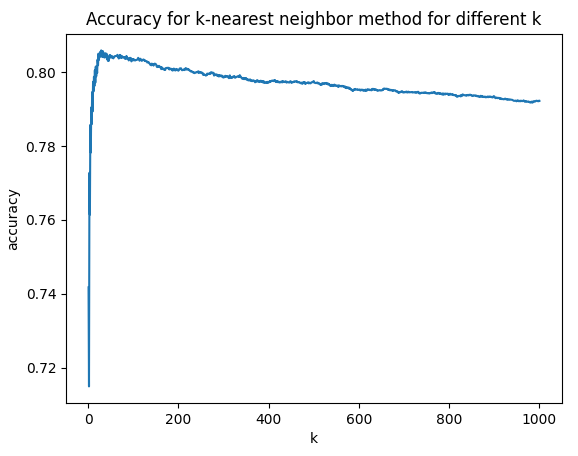
\includegraphics{knn_accuracy.png}
% }
% \caption{
% \label{knn-accuracy}
% }
% \end {center}
% \end {figure}

For this value (k = 29) classes are further predicted already for the real test data.

\begin{figure}[htp] 
    \centering
    \subfloat[a]{%
        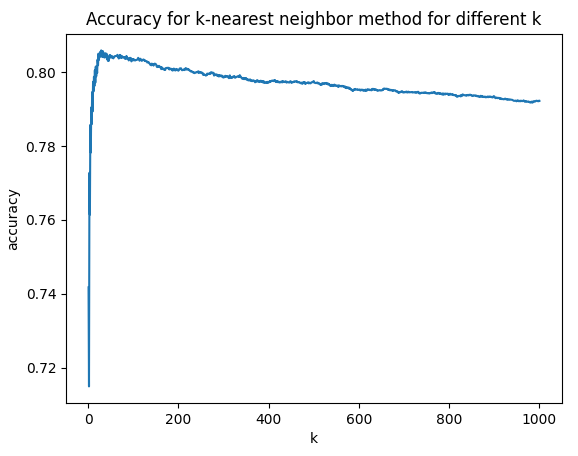
\includegraphics[width=0.22\textwidth]{knn_accuracy.png}%
        \label{fig:a}%
        }%
    \hfill%
    \subfloat[b]{%
        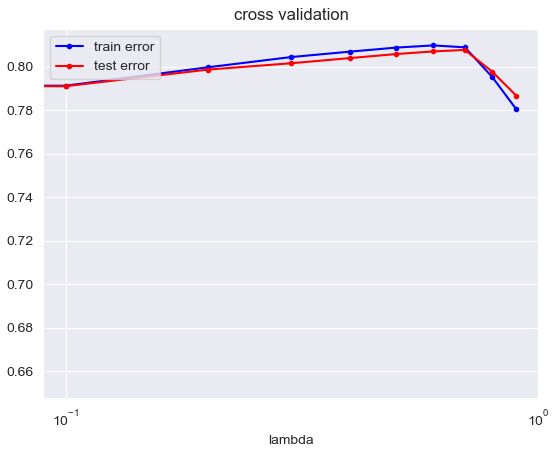
\includegraphics[width=0.22\textwidth]{gamma.png}%
        \label{fig:b}%
        }%
    \caption{Accuracy plot for Knn [a] and Logistic Regression [b] methods on cross validation depending on the values of k and lambda respectively}
\end{figure}



\item {\textit{Logistic Regression}.}

It is transparent that the most appropriate model to use is Logistic Regression which satisfies our classification task. And in practice, it works faster than KNN. 
We attempted both Logistic Regression with and without regularisation. In most cases, our model didn't overfit, as shown below. So eventually, we have chosen the Logistic Regression without regularization as our main model to work on.

Since we needed to specify hyperparameters, which is the step size($\gamma$) for gradient descent and degree of polynomial feature expansion, we used Grid Search to find optimal values in 2-fold Cross-Validation to get the best accuracy score. (best gamma $\approx$ 0.7 for 4000 iterations, best degree = 2)
But ultimately, we came up with an idea to reduce the step size for each 10 000th iteration(out of 40 000, so we used the step size of whatever we prefer with degree 2 to get to the optimal solution eventually.

The train and test accuracy results are presented in the following table for Logistic Regression and KNN.

\begin{center}
\begin{tabular}{||c c c||} 
 \hline On the validation set: \\ \hline\hline
 Model & Train Accuracy & Test Accuracy \\ [0.5ex] 
 \hline\hline
 KNN & 0.80592 & 0.808 \\ 
  Logistic Regression & 0.816035 & 0.8135 \\ 
  \hline
 \hline In the platform: \\ \hline\hline
  Model & Accuracy & F1 Score \\ [0.5ex] 
  \hline\hline
  KNN & 0.808 & 0.711 \\ 
  Logistic Regression & 0.812 & 0.715 \\ 
  \hline
 \end{tabular}
\end{center}
\hfill \break
The numbers above were produced by splitting the training dataset into two parts (one for training and another for validation) and applying data preprocessing.
Another table will show the efficiency of our models submitted to the online platform \href{AICrowd}{https://www.aicrowd.com/} to validate the prediction of the test dataset.

Observing the results, we can conclude that Logistic Regression performs better and faster in comparison to KNN.
\end{enumerate}
\subsection{Possible methods to improve our accuracy:}
\begin{enumerate}
    \item {As our dataset is unbalanced and in this problem, it is crucial to classify "Higgs boson", Random Forest Classifier could possibly be a better solution with its penalization of misclassifying the minority class.}
    \item {It would be interesting to try to feed to one model just "raw" features and to another one  - variables computed by physicists. Eventually, the final model will summarize the predictions of the two previous ones.}
    \item {Since we consider only 20 possible gammas and 3 possible degrees, it is not enough for getting truly optimal hyperparameters. A possible solution for it would be the Optuna optimization framework that in fact optimizes hyperparameters.}
\end{enumerate}
\section{Summary}
This project shows explicitly why preprocessing is so important. We went through the main strategies to improve our model and got the result of percentage of accuracy 81 with Logistic regression. But we still believe that there is a lot to discover in this problem, especially using more advanced techniques. 

\begin{thebibliography}{9}
\bibitem{lamport94}
  Feature Transformation\\
  \textit{\url{https://www.analyticsvidhya.com/blog/2020/07/types-of-feature-transformation-and-scaling/}}
\bibitem{lamport94}
  Feature Engineering\\ \textit{\url{https://machinelearningmastery.com/discover-feature-engineering-how-to-engineer-features-and-how-to-get-good-at-it/}}
\bibitem{lamport94}
  One-Hot-Encoding\\
  \textit{\url{https://vitalflux.com/one-hot-encoding-concepts-python-code-examples/}}
\end{thebibliography}
\end{document}
